\section{Calibration of the Electronic and Nuclear Recoil Bands}
\label{secBandCalibration}

The discrimination efficiency based on the ratio of the prompt and proportional scintillation signals is energy-dependent, and the distributions (so-called `bands') of electronic and nuclear recoils must be calibrated. 
These calibrations have been performed and with Compton-scattered $\gamma$-rays from a $^{60}$Co source, and with neutrons from an $^{241}$Am-Be source, respectively. The electronic recoil data has been acquired regularly with the calibration source placed in the copper pipe around the detector, and consists of 5.8 live days in total. The nuclear recoil calibration data with the total live time of 2.9~days has been acquired in Fall 2009, at the time of the commissioning run. In order to shield the detector from 4.4~MeV $\gamma$-rays from de-excitation of the $^{12}$C isotope, a lead brick has been installed inside the shield (see Fig.~\ref{figXe100shield_1} and Fig.~\ref{figDetectorModel}), and the $^{241}$Am-Be source was placed behind about 5~cm of lead. 

The discrimination parameter log$_{10}$(S2/S1) has been constructed using the summed S2 signal of the bottom PMTs, due to more uniform distribution and smaller uncertainty from the spatial corrections (Section~\ref{secLCEs2}). The electronic recoil and nuclear recoil bands are shown in log$_{10}$(S2/S1) space in Fig.~\ref{figRun07bands}.

\begin{figure}[!h]
\centering
\subfigure[electronic recoils]{
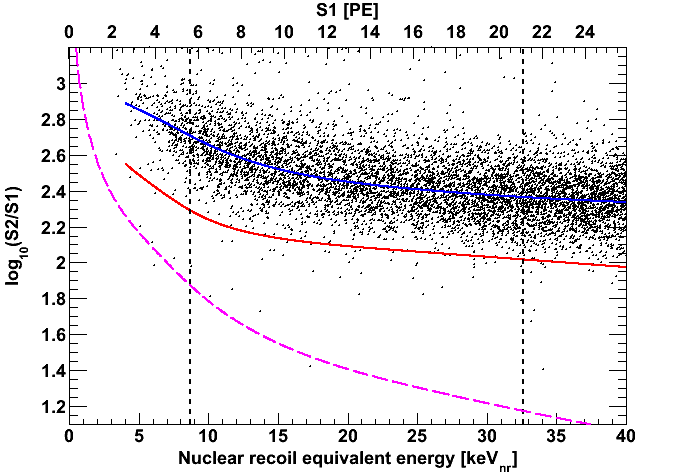
\includegraphics[width=0.475\linewidth]{plots/run07/run07_bandER1.png}
\label{figRun07bands_1}}
\subfigure[nuclear recoils]{
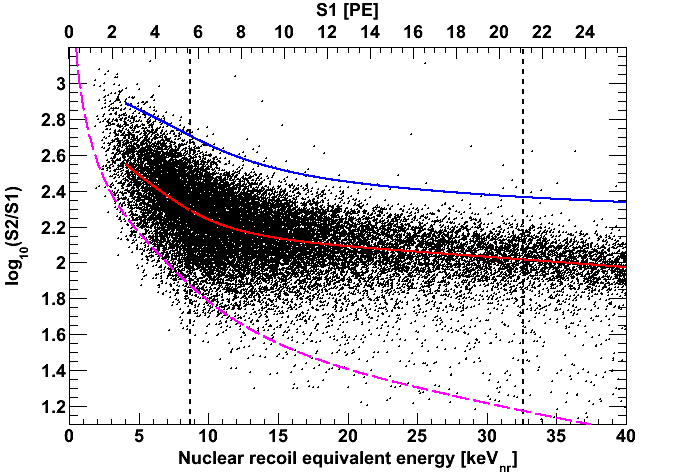
\includegraphics[width=0.475\linewidth]{plots/run07/run07_bandNR1.png}
\label{figRun07bands_2}}
\caption[Electronic recoil and nuclear recoil bands for the analysis of run07 data]{Electronic recoil (a) and nuclear recoil (b) bands for the analysis of run07 data, calibrated with the $^{60}$Co and $^{241}$Am-Be sources, respectively. The median of the electronic recoil band is shown with the blue line, and the median of the nuclear recoil band with the red line. The energy region for WIMP-search is indicated with the dashed black lines. The dashed magenta lines shows the software S2 energy threshold used for the analysis. The vertical  dashed lines show the energy region 8.7-32.6~keV$_{\mathrm{nr}}$, used for the analysis of run07 data.}
\label{figRun07bands}
\end{figure}

For the analysis of first science run data (run08), the bands have been flattened by subtracting the mean of the electronic recoil band, which has been parametrized with a 9th order polynomial function (see Fig.~\ref{figRun08log10signal_1} for background data).

The signal region for run07 analysis has been defined at constant 50\% nuclear recoil acceptance a 8.7$-$32.6~keV$_{\mathrm{nr}}$ energy region (see Fig.~\ref{figCutsAcceptance_1}). The corresponding electronic recoil rejection is above 99\%, and the cumulative acceptance of the data quality cuts varies in this range from 60\% to 85\% (see Section~\ref{secDataQualityCuts}).

For the run08 analysis, the WIMP-search region has been defined at constant 99.75\% electronic recoil rejection, due to an increased level of electromagnetic background in respect to run07 (see Section~\ref{secDataMCcomparison}). 
The electronic recoil band is well described by a Gaussian distribution in the log$_{10}$(S2/S1) and the flattened parameter space. This feature is used to predict the Gaussian leakage, based on the number of events in the WIMP-search data outside the blinded signal region.

%\begin{equation}
%2.93418854
%-0.251661194 \cdot S1
%0.03922036 \cdot S1^2
%-0000200455-0.00357708 \cdot S1^3
% \cdot S1^4
% \cdot S1^5
% \cdot S1^6
% \cdot S1^7
% \cdot S1^8
% \cdot S1^9

%(2.66695+0.267047+0.00019154,
%-0.0960315-0.155731+0.000101306,
%0.00604496+0.0331754,
%-0000200455-0.00357708,
%3.29415e-06+0.000222689,
%-2.10034e-08-8.49461e-06,
%2.01609e-07,
%-2.8995e-09,
%2.30693e-11,
%-7.76065e-14);
%\label{}


%TF1 *ebandfinal = new TF1("ebandfinal","pol9",2,50);
%ebandfinal->SetParameters


%(2.66695+0.267047+0.00019154,-0.0960315-0.155731+0.000101306,0.00604496+0.0331754,-0000200455-0.00357708,3.29415e-06+0.000222689,-2.10034e-08-8.49461e-06,2.01609e-07,-2.8995e-09,2.30693e-11,-7.76065e-14);